\textbf{(a) Modify program $ssq1$ by adding the capability to compute (1) the maximum
delay, (2) the number of jobs in the service node at a specified time (known at a compile time), and (3) the proportion of jobs delayed.\\\\}

\begin{lstlisting}[style=CStyle]

/**
 * Modified February 4, 2023 by hlsun
 * sun.har@northeastern.edu
 * 
 * Added            : Calculations for (1) Maximum Delay, (2) Number of jobs at a given time, (3) Proportion of jobs delayed.
 * Changed          : Changed language from C to C++. Changed to use terminal arguments.
 * Compile with     : g++ -Wall -o Homework2.1 Homework2.1.cpp
 */


/* -------------------------------------------------------------------------
 * This program simulates a single-server FIFO service node using arrival
 * times and service times read from a text file.  The server is assumed
 * to be idle when the first job arrives.  All jobs are processed completely
 * so that the server is again idle at the end of the simulation.   The
 * output statistics are the average interarrival time, average service
 * time, the average delay in the queue, and the average wait in the service 
 * node. 
 *
 * Name              : ssq1.c  (Single Server Queue, version 1)
 * Authors           : Steve Park & Dave Geyer
 * Language          : ANSI C
 * Latest Revision   : 9-01-98
 * Compile with      : gcc ssq1.c 
 * ------------------------------------------------------------------------- 
 */

#include <stdio.h>   
#include <stdlib.h> 

#define FILENAME    "ssq1.dat"                  /* input data file */
#define TIMESET     400.0                       /* time at which number of jobs in the service node is calculated */
#define START       0.0

/* =========================== */
    double GetArrival(FILE *fp)                 /* read an arrival time */
/* =========================== */
{ 
    double a;

    fscanf(fp, "%lf", &a);
    return (a);
}

/* =========================== */
    double GetService(FILE *fp)                 /* read a service time */
/* =========================== */
{ 
    double s;

    fscanf(fp, "%lf\n", &s);
    return (s);
}

/* ============== */
    int main(int argc, char* argv[])
/* ============== */
{
    FILE   *fp;                                  /* input data file      */
    long   index     = 0;                        /* job index            */
    double arrival   = START;                    /* arrival time         */
    double delay;                                /* delay in queue       */
    double service;                              /* service time         */
    double wait;                                 /* delay + service      */
    double departure = START;                    /* departure time       */
    struct {                                     /* sum of ...           */
    double delay;                              /*   delay times        */
    double wait;                               /*   wait times         */
    double service;                            /*   service times      */
    double interarrival;                       /*   interarrival times */
    } sum = {0.0, 0.0, 0.0};

    double MaxDelay = 0;                         /* This variable stores the maximum delay.  */
    int numJobsAtT = 0;                          /* This variable stores the number of jobs at a given time. */
    int timeT = (int) TIMESET;                   /* This variable stores the time at which to calculate numJobsAtT. */
    int numJobsDelayed = 0;                      /* This variable stores the number of jobs delayed. */

	/* If filename is specified as a terminal argument, use that. Else, use the default filename. */
	fp = (argc > 1) ? fopen(argv[1], "r") : fopen(FILENAME, "r");
    
	/* If time is specified as a terminal argument, use that. Else, use the default time. */
	timeT = (argc > 2) ? atoi(argv[2]) : timeT;

    if (fp == NULL) {
    fprintf(stderr, "Cannot open input file %s\n", FILENAME);
    return (1);
    }

    while (!feof(fp)) {
    index++;
    arrival      = GetArrival(fp);
    if (arrival < timeT)
		numJobsAtT++;   /* Increment the number of jobs if it arrives before timeT */
    if (arrival <= departure)
    {
        delay = departure - arrival;        /* delay in queue    */
		numJobsDelayed++;                   /* Increment the number of jobs delayed. */
    }
    else 
        delay      = 0.0;                        /* no delay          */
    service      = GetService(fp);
    wait         = delay + service;
    departure    = arrival + wait;             /* time of departure */
	if (departure <= timeT)
		numJobsAtT--;   /* Decrement the number of jobs if it departs before timeT */
    sum.delay   += delay;
    sum.wait    += wait;
    sum.service += service;
    /* If the delay is greater than the previous maximum delay, store it as MaxDelay. */
    if (delay > MaxDelay)
    {
        MaxDelay = delay;
    }
    }
    sum.interarrival = arrival - START;

    printf("\nfor %ld jobs\n", index);
    printf("   average interarrival time \t= \t%6.2f\n", sum.interarrival / index);
    printf("   average service time .... \t= \t%6.2f\n", sum.service / index);
    printf("   average delay ........... \t= \t%6.2f\n", sum.delay / index);
    printf("   average wait ............ \t= \t%6.2f\n", sum.wait / index);

    printf("   maximum delay ........... \t= \t%6.2f\n", MaxDelay);
    printf("   number of jobs at t = %d  \t= \t%6.1d\n", timeT, numJobsAtT);
    printf("   proportion of jobs delayed\t= \t%6.2f\n", (double) numJobsDelayed / index);

    fclose(fp);
    return (0);
}

\end{lstlisting}
\vspace{20pt}
\noindent Terminal Output:\\\\

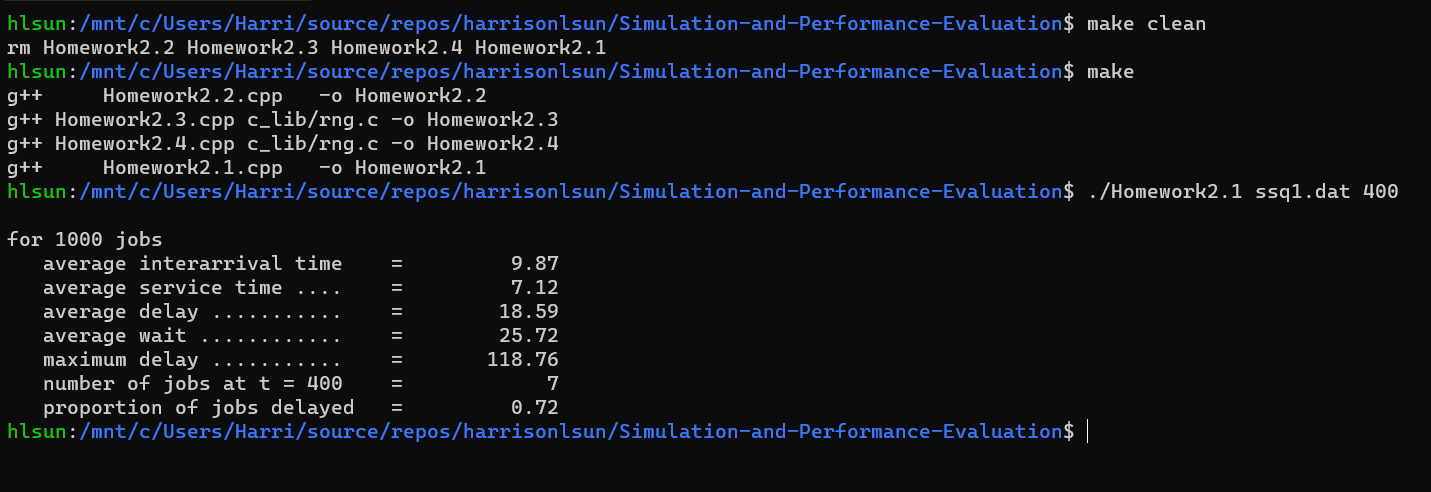
\includegraphics[scale = 0.5]{Sections/H2_1.png}
\newpage
